\begin{figure}[H]
\centering
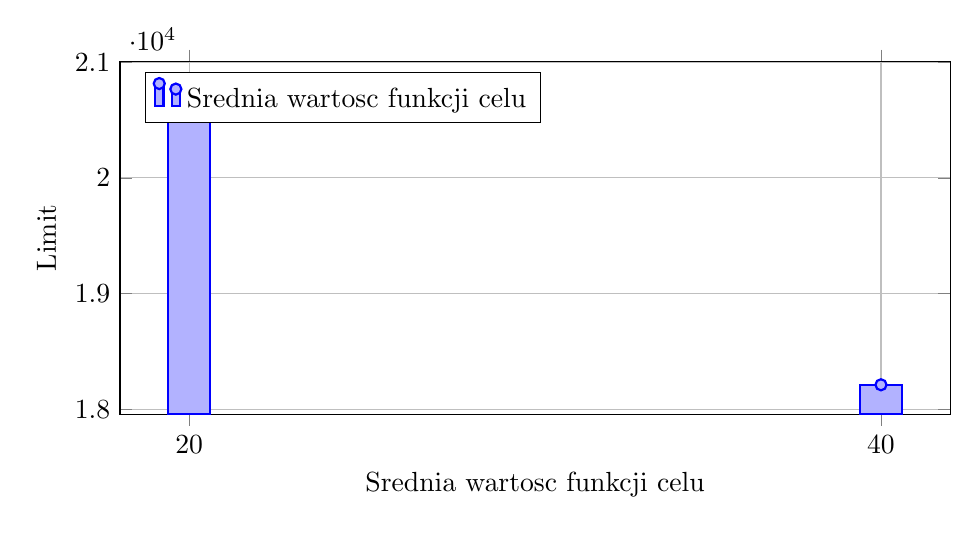
\begin{tikzpicture}
\begin{axis}[
xlabel = {Srednia wartosc funkcji celu},
ylabel = {Limit},
legend pos = north west,
grid = both,
width=1\linewidth,
height=0.5\linewidth,
ybar,
bar width=15pt,
symbolic x coords={20,40,},
xtick=data
]
\addplot + [mark = *, thick] coordinates
    {
(20,20753.125)(40,18210.791666666668)};
\addlegendentry
{Srednia wartosc funkcji celu}
\end{axis}
\end{tikzpicture}
\caption
{Srednia wartosc funkcji celu w zaleznosci od limitu dla wszystkich instancji}
\label{fig:mean_goals_per_limit_all_instances}
\end{figure}
